
\section{Busqueda del PCA y kNN óptimo}

En esta sección diseñamos experimentos para encontrar parametros óptimos  de kNN y PCA de la herramienta de OCR implementado. Para poder hacer esto utilizamos K-fold cross validation.
Como el tiempo de computo de los algoritmos son altos primero hicimos una exploración manualmente con algunos parametros dispersos con el fin de acotar el espacio de busqueda. Las metricas que utilizamos para analizar que tan bien se reconocen los caracteres.



\subsection{Hipótesis}
Para el algoritmo de KNN, nuestra hipotesis es que para los valores mas bajos de k la cantidad de aciertos sera menor porque para caracteres similares una imagen puede tener algunos vecinos cercanos de otra clase. Para valores muy grandes de k se consideran demasiados digitos y en este caso toma mas importancia a la cantidad de apariciones de un caracter que la cercania de los miembros de su clase. Un ejemplo para ilustrar este comportamiento es cuando k toma su valor maximo, la cantidad total de datos de entrenamiento, la repuesta siempre sera la clase que tenga mas elementos en la base de entrenamiento.

Para los algoritmos del método PCA, nuestra hipotesis es que la calidad de nuestos resultados crece junto con el valor de alpha, aunque creemos que va a existir un punto b en el cual los resultados no van tener mejoras significativas. Creemos que esto se debe a que proyectamos el espacio original a otro generado por los autovectores asociados a los mayores autovalores asi se preserva la mayor cantidad de información en las primeras b columnas de la matriz transformada.

\subsection{Con parametros dispersos}

Como ya dicho anteriormente seleccionamos parámetros dispersos para poder encontrar los parametros optimos utilizando kNN con PCA, nuestra elección para los k y los alpha fueron [1,5,10,30,50,100], estos numeros los tomamos cada vez mas grandes por el simple hecho de que el costo de tiempo es mayor y ademas porque creemos que no se van a conseguir mejoras significativas o bien seran resultados negativos. Ademas el K lo tomaremos en 5 que nos pareció un buen punto de partida.

\subsubsection{Resultado}




\subsubsection{Análisis de resultado}
A partir de estos resultados podemos observar que sorprendentemente con k=1 fueron bastante positivos pero no los mejores, esto nos parecio destacable ya que pensabamos que iba a ser poco probable que el mas cercano, generalmente, sea el correcto. También se encuentra entendible que los valores mayores de k decrece su eficacia rapidamente viendo como razón la hipotesis dada.

Para los alpha se encontró que la hipotesis se cumple, ya que los primeros valores tienen resultados muy negativos y a partir de la variable 30 se encuentra este punto b del que hablabamos. Particularmente con el alpha mayor se encuentra un decrecimiento breve, a lo que lo asociamos con algunos problemas de redondeo y arrastres de errores.

Por lo tanto para el próximo experimento, el que será mas riguroso, tomaremos el intervalo de k=[2, ... , 7] y alpha=[25, ... , 40]. 

\subsection{Tomando mas rigurosidad}

\subsubsection{Resultados}


\subsubsection{Análisis de resultados}



\section{Variando tamaño del set de entrenamiento}

En esta parte probaremos distintos k para distintos tamaños de set de entrenamiento, para poder observar si se encuentra alguna diferencia entre los tamaños y su k en kNN.
Para poder ver esto, tomamos la misma cantidad de imágenes de cada clase aleatoriamente. Los tamaños elegidos fueron [5000, 10000, 20000, 30000, 42000], la variable $\alpha$ la mantuvimos como la optima que se obtuvo en el experimento anterior, el k se utilizo entre[1, 5, 10, 20, 50, 75, 100] y el K de K-fold lo mantuvimos en 5.

\subsection{Hipótesis}

Nuestra hipótesis sera que a medida que el tamaño del set de entrenamiento decrece y mientras el k crece, los resultados decrecerán estrepitamente. En primer lugar si el k crece, como fue demostrado en el experimento anterior, veremos disminuciones en la eficacia. En segundo lugar, mientras el set de entrenamiento se achica, se tendrán menos datos para entrenar y el algoritmo de kNN tomara muchos valores, lo cual terminara resultando en una mala predicción.

\subsection{Resultados}


\begin{center}
   \includegraphics[caca][scale=0.6]{graficos/Accuracy_distintos_tamanos.png}
   \label{Fig. 2}
\end{center}

\begin{center}
   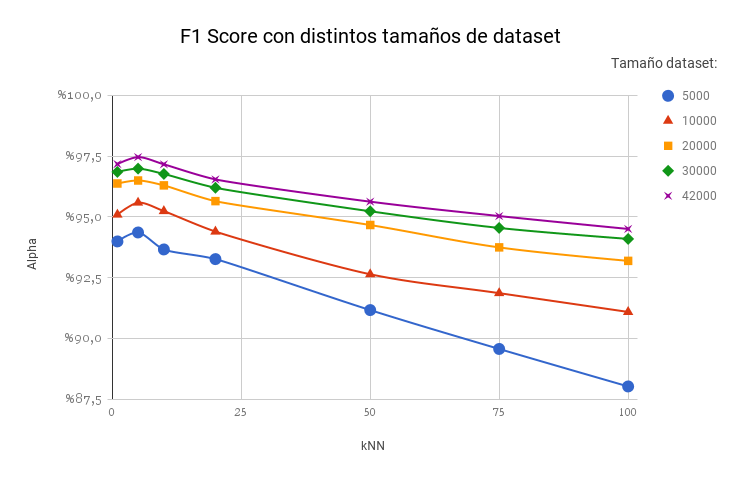
\includegraphics[scale=0.6]{graficos/F1_score_distintos_tamanos.png}
   \label{Fig. 1}
\end{center}

\subsection{Análisis de los Resultados}

A partir de este resultado podemos reafirmar la hipótesis del experimento anterior y se pude decir que se cumplió con lo esperado, ya que al disminuir la cantidad de imágenes de entrenamiento, tanto el accuracy como el f1 score bajan. Tambien se observa que con con k muy altos, para el caso de 5000 imágenes, el porcentaje baja linealmente, lo cual cumple con lo que decíamos.